\documentclass[12pt]{article}

\usepackage{xcolor}
\usepackage{float}
\usepackage{graphicx}
\usepackage{fancyhdr}

\usepackage[utf8]{inputenc}
\usepackage{setspace}

\usepackage[dvips,letterpaper,margin=1in]{geometry}

\setlength{\parindent}{0pt}
\setlength{\headheight}{15pt} % fancyhdr wants at least 14.5pt

% Header
\pagestyle{fancy}
\lhead{MFRFS K3 XPedite-7674 Interface Discussion}
\rhead{June 23, 2020}
\renewcommand{\headrulewidth}{0.4pt}
\renewcommand{\footrulewidth}{0.4pt}

% Start document
\begin{document}

%%%%%%%%%%%%%%%%%%%% Title Page %%%%%%%%%%%%%%%%%%%%%%%%
\thispagestyle{empty}
\begin{titlepage}
\begin{center}
        \vspace*{1cm}

        \LARGE{Multi-Function Radio Frequency System (MFRFS) K3 \\
            XPedite-7674 Interface Discussion}

        \vspace{0.5cm}
        \LARGE
        % Subtitle

        \vspace{1.5cm}

        \normalsize

        John Jesus \\
        June 23, 2020

        \vfill



        \vspace{0.8cm}




\end{center}
\end{titlepage}

\tableofcontents
\newpage

%%%%%%%%%%%%%%%%% Start of Body %%%%%%%%%%%%%%%%%%%%%%%%
\section{Scope}
\subsection{Purpose}
This document is to guide a discussion of a subset of the interfaces on the XES Xpedite7674 Single Board Computer as planned for MFRFS K3.

\subsection{References}
\begin{enumerate}
    \item XPedite7674 Users Manual Revision C (Extreme Engineering Solutions, February 1, 2018)\label{ref:1}
    \item System Controller Unit, MBA Schematic Diagram (Raytheon Drawing \#SDD0862530 Initial Revision)\label{ref:2}
\end{enumerate}

\section{Interfaces}
Interfaces are depicted in Figure \ref{fig:inteface}; this image was created by Cody Jeffcoat of Raytheon McKinney and derived from the vendor document of Reference \ref{ref:1} and the Raytheon schematic drawing of Reference \ref{ref:2}. Markings were added to aid in the discussion of the interfaces.

\begin{figure}[H]
\begin{center}
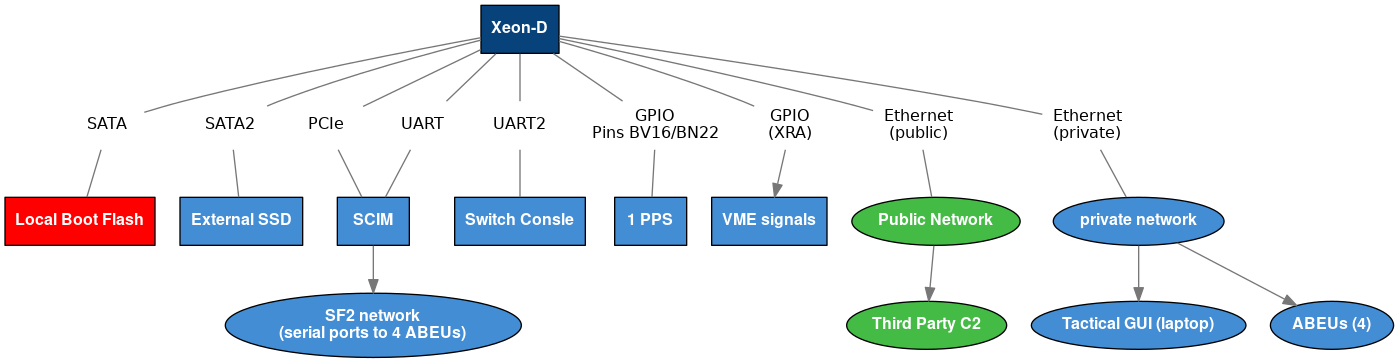
\includegraphics[width=1.0\textwidth]{img/interface}
\caption{MFRFS K3 SCU SBC-0 Xpedite7674}
\label{fig:inteface}
\end{center}
\end{figure}

\end{document}

